\secnumbersection{PROPUESTA DE SOLUCIÓN}

% En esta sección (??)

\subsection{Metodología de trabajo}
\label{sec:metod-de-trabajo}

Para nuestro proyecto, buscaremos utilizar una metodología de trabajo orientada a la agilidad. Existen multiples metodologias de este estilo, pero hemos decidido utilizar el ciclo \textit{PDCA}\footnote{PDCA: Del inglés Planear, Hacer, Verificar, Actuar.} (\textit{Plan}, \textit{Do}, \textit{Check}, \textit{Act}) por las siguientes razones.

\begin{itemize}
    \item \textbf{Simple}. Nuestro mayor motivo es que consiste en un proceso simple, directo e intuitivo que podemos adoptar e implementar en nuestro flujo de trabajo, desarrollo e implementación de la solución.
    \item \textbf{Cilcico}. Debido a la naturaleza ciclica e iterativa, \textit{PDCA} nos permite identificar las causas de los posibles errores durante el proceso de desarrollo del proyecto. Además, a medida que se implementan distintas soluciones es posible obtener información y experiencia para comprender el proceso que se busca mejorar.
    \item \textbf{Adaptable}. Esta metodología es una estrategia muy adaptable, aquellas personas que decidan implementarla puede decidir con total libertad que aspectos se deben considerar en cada una de las etapas del ciclo, la unica condición es que las definiciones se deben mantener a lo largo de todo el proceso. Esta adaptabilidad permite que \textit{PDCA} sea altamente esacalable, ya que se puede adaptar a cualquier situación y en organizaciones de cualquier tamaño, incluso, en equipos de una sola persona.
\end{itemize}

\begin{figure}[ht]
    \centering
    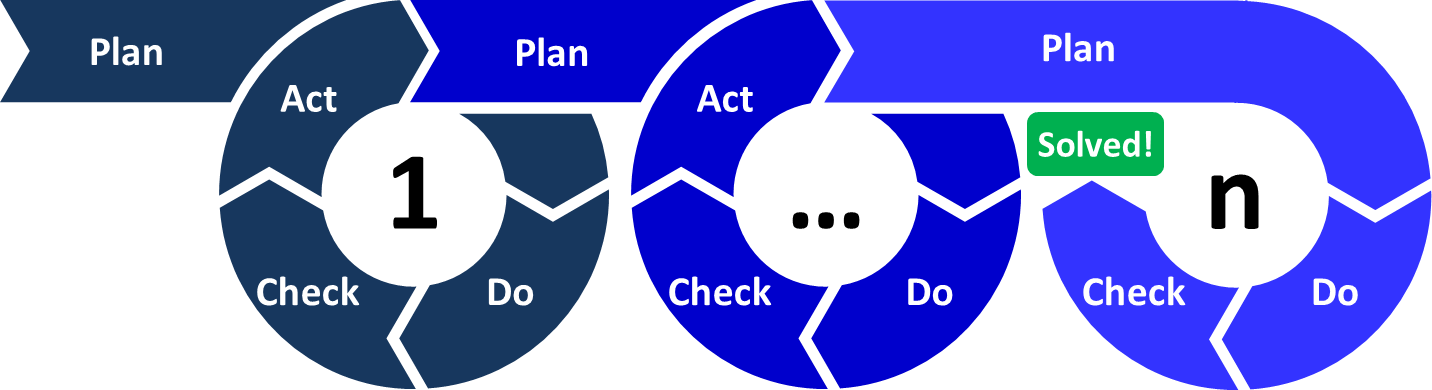
\includegraphics[width=\linewidth]{PDCA-Multi-Loop.png}
    \caption{Ciclos \textit{PDCA}.} Multiples iteraciones del ciclo \textit{PDCA} son realizadas hasta que se logra resolver el problema. Fuente: \textit{PDCA - Wikipedia Commons}.
    \label{fig:pdca-cycle}
\end{figure}

En su esencia \textit{PDCA} es una filosofía para abordar problemas. Primero, identificamos el problema y establecemos nuestros objetivos. Luego, probamos distintos enfoques para alcanzar dichos objetivos, analiszamos nuestros resultados y adaptamos nuestro comportamiento en base a estos. Finalmente, avanzamos la iteración utilizando la solución que ha funcionado.
% TODO: FIXME: REF to https://www.dropbox.com/es/business/resources/pdca

Cada ciclo \textit{PDCA} consiste en las siguientes etapas.

\begin{itemize}
    \item \textbf{Planear}. Debemos comprender nuestro estado actual y el estado deseado. En pocas palabras, esta estapa busca que definamos nuestros objetivos, el cómo alcanzarlos y cómo medir nuestro progreso hacia dichos objetivos.
    \item \textbf{Hacer}. Una vez que hemos definido un plan de acción o una potencial solución para un problema, debemos probarla. Este paso es donde debemos poner a prueba los cambios propuestos en la etapa Planear. Sin embargo, esto se debe considerar como un experimento, no como una solución final. Por lo tanto, todas las pruebas se deben realizar en entornos controlados y a pequeña escala.
    \item \textbf{Verificar}. Luego de completar nuestras pruebas, debemos comprobar que los cambios o soluciones propuestas tienen el efecto deseado. En esta etapa se debe analizar la información recopilada durante la etapa Hacer y comparar lo obtenido con los objetivos y metas originales. En resumen, debemos evaluar nuestro nivel de éxito y qué cosas vamos a conservar para el siguiente paso del ciclo.
    \item \textbf{Actuar}. Al llegar a esta etapa, ya hemos logrado identificar una solución o propuesta de cambio para implementar en nuestro problema o proceso. Se deben aplicar estos cambios en la escala que sea necesaria por el proceso y con esto se definen las bases para una nueva iteración.
\end{itemize}

\subsection{Plan de trabajo}
\label{sec:plan-de-trabajo}

Como hemos mencionado anteriormente, vamos a utilizar cilcos \textit{PDCA} para encontrar la solución a nuestro problema, estos ciclos, son definidos conforme avanzamos en las iteraciones y debido a que se encuentra en el marco de las metodologias agiles, seria irresponsable definir con antelación los objetivos de cada ciclo. Sin embargo, podemos definir determinados hitos que buscamos lograr durante todo este proceso, los cuales, detallamos a continuación.

\begin{enumerate}
    \item Entender la arquitectura inicial de la solución existente (\textit{SPARQLforHumans}).
    \item Diseñar y definir una arquitectura acorde a nuestras restricciones.
    \item Reducir significativamente el tiempo necesario para ejecutar la solución.
    \item Diseñar y definir una arquitectura que permita la actualización en tiempo real de los datos utilizados por nuestra solución.
    \item Actualizar los datos de nuestra solución en tiempo real.
    \item Validar la solución a través de pruebas unitarias automatizadas.
\end{enumerate}

Estos hitos, nos permitiran guiar las iteraciones de nuestro proceso \textit{PDCA} y así no perder el rumbo durante la implementación.

Con las definiciones realizadas en las secciones \ref{sec:metod-de-trabajo} y \ref{sec:plan-de-trabajo} tenemos los necesario para comenzar nuestras iteraciones.

\subsection{Primera iteración: Analisis inicial de la solución existente}

\subsubsection*{Planificación}

Para nuestra primera iteración, nuestro objetivo es entender el proceso y los componentes de la aplicación \textit{SPARQLforHumans}, para esto, revisaremos el código fuente disponible de forma publica \cite{parra2020autocompletion}.

\subsubsection*{Implementación}

Comenzaremos con entender el proceso. Al revisar el código fuente de la aplicación, logramos identificar las siguientes etapas.

\begin{enumerate}
    \item Inicio de la aplicación.
    \begin{enumerate}
        \item Lectura de un fichero en el formato de compresión \textit{gzip} \cite{rfc1952} desde \textit{Wikidata}.
        \item Filtro y validación de lineas en formato \textit{N-Triples}.
        \item Creación de objetos \textit{Triple} en base a lineas validas.
        \item Generación de propiedades inversas para determinadas entidades.
        \item Concatenación de lineas validas y nuevas propiedades a nuevo fichero \textit{gzip}.
        \item Ordenar lineas de nuevo fichero en función de la entidad \textit{RDF} observada en cada linea.
    \end{enumerate}
    \item Indexación de entidades.
    \begin{enumerate}
        \item Lectura de nuevo fichero \textit{gzip} generado anteriormente.
        \item Creación de objetos \textit{Triple}.
        \item Generación de documentos en indice \textit{Lucene} en base a propiedades de cada entidad.
    \end{enumerate}
    \item Obtención del valor \textit{PageRank} para entidades.
    \item Indexación de propiedades.
    \begin{enumerate}
        \item Lectura de documentos disponibles en indice \textit{Lucene} para entidades.
        \item Calculo de frecuencias para las propiedades existentes en los distintos documentos.
        \item Generación de documentos en nuevo indice \textit{Lucene} en función de la frecuencia de cada propiedad identificada.
    \end{enumerate}
    \item Sistema en vivo.
    \begin{enumerate}
        \item Ejecución de prueba estadistica y de rendimiento.
        \item Inicio de servidor Web.
    \end{enumerate}
\end{enumerate}

Las interacciones entre cada etapa se puede observar en el diagrama de procesos presentado en la figura \ref{fig:sfh-bpmn} y los componentes identificados se pueden observar en la figura \ref{fig:sfh-componentes}.

\begin{figure}[ht]
    \centering
    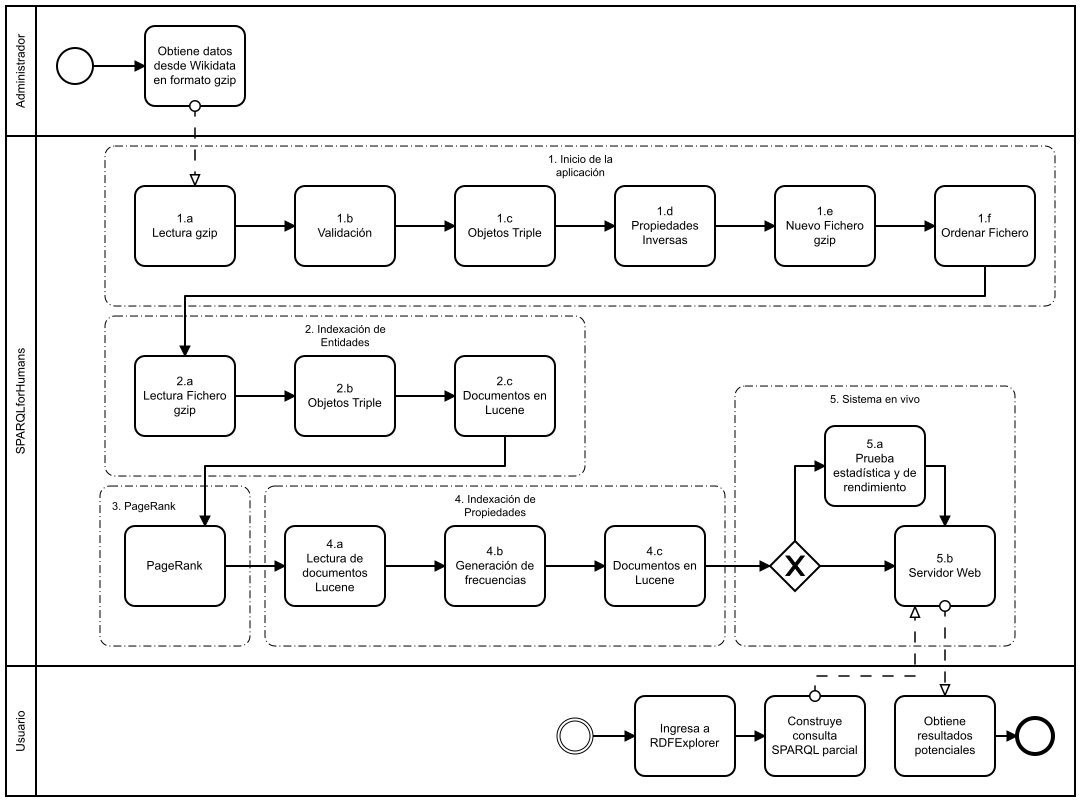
\includegraphics[width=\linewidth]{sparqforhumans_process_bpmn}
    \caption{Proceso de arranque de la aplicación \textit{SPARQLforHumans}.}Fuente: Elaboración Propia.
    \label{fig:sfh-bpmn}
\end{figure}

\begin{figure}
    \centering
    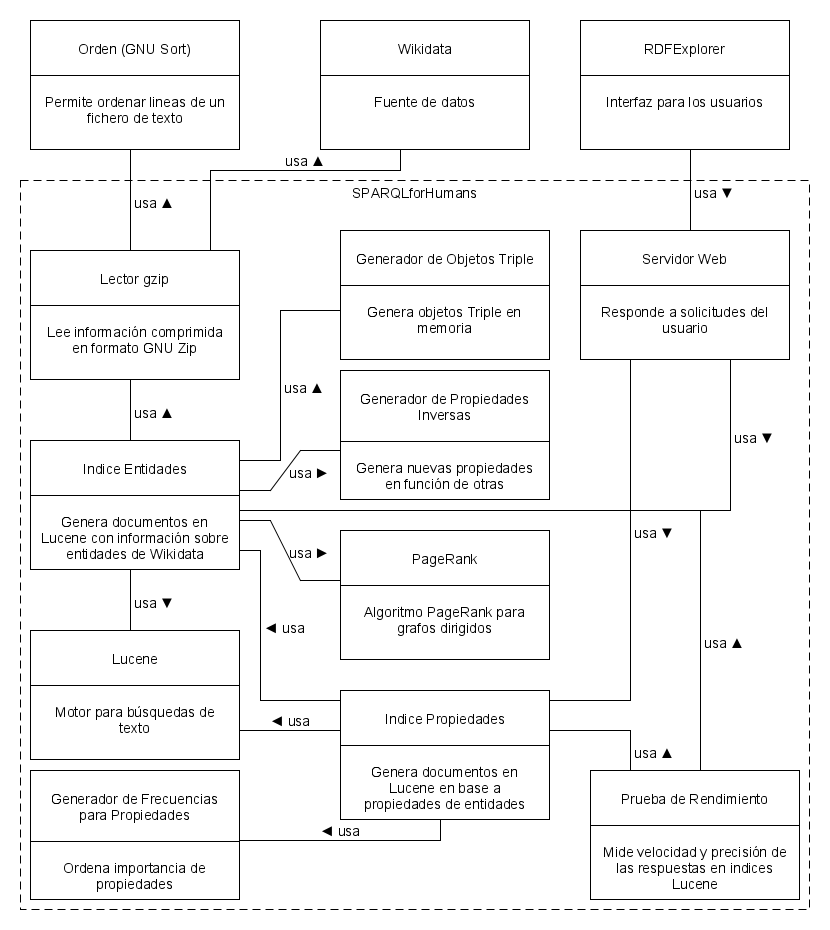
\includegraphics[width=\linewidth]{sfh_comm}
    \caption{Diagrama de componentes para la aplicación \textit{SPARQLforHumans}.}Fuente: Elaboración Propia.
    \label{fig:sfh-componentes}
\end{figure}

\subsubsection*{Resultados}

Gracias al levantamiento de proceso y componentes realizado, podemos ver de forma más clara cómo interactuan cada uno de los distintos modulos de la aplicación existente. Esto nos permite entender su funcionamiento interno, de forma tal, que podemos comenzar a optimizar cada uno de los componentes identificados por separado, acercandonos a nuestro objetivo final.

\subsection{Segunda iteración: Mejoras al rendimiento general}

A

\subsubsection*{Proceso}

A

\subsubsection*{Componentes}

A

\subsubsection*{Diseño inicial de arquitectura}

A

\subsubsection*{Implementación inicial}

A

\subsubsection*{Resultados}

A

\subsection{Tercera iteración: Desacoplamiento de componentes y FlatBuffers}

A

\subsubsection*{Diseño}

A

\subsubsection*{Implementación}

A

\subsubsection*{Resultados}

A

\subsection{Cuarta iteración: Paralelización de etapas}

A

\subsubsection*{Diseño}

A

\subsubsection*{Implementación}

A

\subsubsection*{Resultados}

A

\subsection{Quinta iteración: Actualización de resultados en tiempo real}

A

\subsubsection*{Diseño}

A

\subsubsection*{Implementación}

A

\subsubsection*{Resultados}

A

\subsection{Sexta iteración: Optimizaciones de transporte}

A

\subsubsection*{Planificación}

\subsubsection*{Implementación}

\subsubsection*{Resultados}



\subsection{Septima iteración: Implementación de pruebas}

A

\subsubsection*{Planificación}

\subsubsection*{Implementación}

\subsubsection*{Resultados}

